%\documentclass[a4paper,fleqn,longmktitle]{cas-dc}
\documentclass[a4paper,fleqn]{cas-sc}

%------------------------------------------------------------------------------

% packages
%\usepackage[authoryear,longnamesfirst]{natbib}
\usepackage[authoryear]{natbib}
%\usepackage[numbers]{natbib}
\usepackage{gensymb}
%\usepackage{amsmath} % for centering equations
\usepackage[permil]{overpic} % figure annotations
\usepackage{pict2e} % figure polygon annotations
\usepackage{framed} % Framing content
\usepackage{nomencl} % Nomenclature package
%\usepackage{cuted}
%\usepackage{lineno}
%\usepackage{soul} 
%\usepackage{lipsum}

%------------------------------------------------------------------------------

% macros
\let\WriteBookmarks\relax
\def\figureautorefname{Fig.}
\def\equationautorefname{Eq.}
%\def\tableautorefname{Tbl.}
\def\sectionautorefname{Section}
\def\subsectionautorefname{Subsection}
\def\floatpagepagefraction{1}
\def\textpagefraction{.001}
\newcommand{\f}{\mkern-2mu f\mkern-3mu}

%------------------------------------------------------------------------------

% style
%\bibliographystyle{model1-num-names}
\bibliographystyle{cas-model2-names}
\makenomenclature
\setlength{\nomlabelwidth}{13mm}
\setlength{\nomitemsep}{-\parskip} % Baseline skip between items
% \setlength{\abovecaptionskip}{0pt plus 1.0pt minus 1.0pt}
% \setlength{\textfloatsep}{20pt plus 2.0pt minus 4.0pt}
% \textfloatsep: 20.0pt plus 2.0pt minus 4.0pt;
% \floatsep: 12.0pt plus 2.0pt minus 2.0pt;
% \intextsep: 12.0pt plus 2.0pt minus 2.0pt
% \linenumbers

%------------------------------------------------------------------------------

\begin{document}

% title
\title [mode = title]{Real-time spectral radiance estimation of hemispherical clear skies with machine learned regression models}
\shorttitle{Real-time spectral radiance estimation of clear skies}
% \tnotemark[1]
% \tnotetext[1]{This document is the results of the research
%   project funded by the National Science Foundation.}

% authors
\shortauthors{J. Del Rocco et~al.}
\author[1]{{Joseph} {Del Rocco}}
\cormark[1]
% \fnmark[1]
\ead{jdelrocco@ist.ucf.edu}
% \ead[url]{www.cvr.cc, cvr@sayahna.org}
% \credit{Conceptualization of this study, Methodology, Software}
\author[2]{Paul D. Bourke}
\author[3]{Charles B. Patterson}
\author[1]{Joseph T. Kider}
\address[1]{IST, School of Modeling, Simulation, \& Training, University of Central Florida, Orlando, FL, USA}
\address[2]{University of Western Australia, Crawley WA, Australia}
\address[3]{Full Sail University, Winter Park, FL, USA}

% title footnotes
\cortext[cor1]{Corresponding author.}
% \cortext[cor2]{Principal corresponding author}
% \nonumnote{jdelrocco@ist.ucf.edu (J. Del Rocco)}
% \fntext[fn2]{Another author footnote, this is a very long footnote and
%   it should be a really long footnote. But this footnote is not yet
%   sufficiently long enough to make two lines of footnote text.}
% \nonumnote{This note has no numbers. In this work we demonstrate $a_b$
%   the formation Y\_1 of a new type of polariton on the interface
%   between a cuprous oxide slab and a polystyrene micro-sphere placed
%   on the slab.
%   }

% abstract
\begin{abstract}
Whole sky spectral radiance distribution measurements are difficult and expensive to obtain, yet important for real-time applications of radiative transfer, building performance, physically based rendering, and photovoltaic panel alignment. This work presents a validated machine learning approach to predicting spectral radiance distributions (350-1780 nm) across the entire hemispherical sky, using regression models trained on high dynamic range (HDR) imagery and spectroradiometer measurements. First, we present and evaluate measured, engineered, and computed machine learning features used to train regression models. Next, we perform experiments comparing regular and HDR imagery, sky sample color models, and spectral resolution. Finally, we present a tool that reconstructs a spectral radiance distribution for every single point of a hemispherical clear sky image given only a photograph of the sky and its capture timestamp. We recommend this tool for building performance and spectral rendering pipelines. The spectral radiance of 81 sample points per test sky is estimated to within 7.5\% RMSD overall at 1 nm resolution. Spectral radiance distributions are validated against libRadtran and spectroradiometer measurements. Our entire sky dataset and processing software is open source and freely available on our project website. \footnote{https://spectralskylight.github.io}
\end{abstract}

% \begin{graphicalabstract}
% \includegraphics{figs/grabs.pdf}
% \end{graphicalabstract}

% \begin{highlights}
% \item Research highlights item 1
% \item Research highlights item 2
% \end{highlights}

% keywords
\begin{keywords}
sky radiance \sep spectral radiance \sep all sky \sep machine learning \sep building performance \sep HDR
\end{keywords}

\maketitle

% text
\section{INTRODUCTION}
\label{sec:introduction}

Multispectral sky radiance is needed for wavelength dependent computations in a wide variety of domains and applications, including: radiative transfer,\cite{chandrasekhar_radiative} building-performance simulation,\textsuperscript{\citenum{jakica_survey},\citenum{hensen_buildingperformance}} photovoltaic (PV) panel alignment\cite{smith_tilt}, climate science,\cite{lopez-alvarez_using_2008} physically based rendering\textsuperscript{\citenum{jakob_mitsuba},\citenum{haber_physically}} natural light transport,\textsuperscript{\citenum{veach_metropolis},\citenum{jarosz_montecarlo}} and any thermal/lighting application using bidirectional reflectance distribution functions (BRDFs).\cite{kurt_survey, cook_torrance_brdf, deering_atmospheric, nicodemus_brdf} The spectra ranges of interest can vary based on a number of factors; we use the following: visible (VIS) (380-780nm), visible and near-infrared (VNIR) (380-1400nm), and short wave infrared (SWIR) (1000-2500nm). Of even more importance is the need for collections of whole sky angular dependent radiance distribution curves required for accurate computations on surfaces affected by the angle of incidence, e.g. walls, facades, PV panels, all of which require more than just a single downward-welling radiance measurement, and all of which need to account for occlusions of the visible skydome.\cite{schumann_environment} Despite the fact that skylight itself has been studied for well over one hundred years (going back to Lord Rayleigh\cite{strutt_lightfromsky_1871}, Mie\cite{mie_beitrage_1908}, Kimball\cite{kimball_intensity}, and Pokrowski\cite{pokrowski_1929}, to name a few), the process of actively measuring or even computing whole sky radiance distributions quickly and accurately still remains an open problem, especially if the curves are to be used in a real-time, practical setting. Reliable, fast, cost-effective methods are still desired. This work attempts to use various modern machine learning methods to train models with the express purpose of being used in a real-time setting to estimate whole sky radiance curves quickly, within some acceptable error, using a dataset of whole sky images and radiance distributions measured with a custom-built hardware system.\cite{kider_framework_2014}

% \begin{figure}[btp]
% \begin{center}
% \includegraphics[width=1.0\textwidth,height=0.25\textwidth]{img/intro_vns.jpg}
% \end{center}
% \caption{\label{fig:spectrum}Sky radiance distribution spectra of interest: VIS, VNIR, and SWIR.}
% \end{figure}

% Some relevant contributions to this problem in the last decade include the following: Refs. \citenum{saito_estimation_2016, chauvin_modelling_2015, kocifaj_unified_2015, tohsing_validation_2014, cordero_downwelling_2013, roman_calibration_2012, ehrlich_airborne_2012, pissulla_comparison_2009, lopez-alvarez_using_2008, cazorla_using_2008, cazorla_development_2008, lee_jr_measuring_2008, milton_estimating_2006}.

Saito et al. estimated sky radiance distributions with a derived equation taking total ozone column and RAW RGB counts.\cite{saito_estimation_2016} They specifically attempt sky radiance estimation \enquote{without any training sets,}\cite{saito_estimation_2016} but focus on a single point in the sky (the zenith) for a subset of visible wavelengths (430-680nm). An important contribution is their camera-specific color matching functions (CMFs), an extension of work done by Sigernes et al.,\cite{sigernes_sensitivity} which take into account camera lens wavelength dependence, vignetting effect, and CMOS noise.\cite{saito_estimation_2016} 

Tohsing et al. used a machine learning approach to estimate full visible spectrum whole sky radiance distributions. They used non-linear regressions, one per color component (RGB) per wavelength (380-760nm), or 1143 models, using the non-linear relationships between RGB counts and radiance values.\cite{tohsing_validation_2014} Although they use 113 sampled points of the hemisphere, their measurements are limited to 8 of 12 consecutive days of the year, with only 1 day's clear sky data and 1 day's overcast data used for training.\cite{tohsing_validation_2014} They classify sky cover procedurally into 2 groups (clear or cloudy) via sky index,\textsuperscript{\citenum{yamashita_cloud},\citenum{saito_cloud}} and train 2 separate groups of regressions; scattered skies thus use one or the other. Because full hemisphere measurements took 12 minutes to complete, a synchronized, synthetic image was constructed and sampled.

Chauvin et al. also used a custom-built sky viewer/imager to obtain and then remove/clean anisotropy from clear sky portions of sky images for better cloud detection and ultimately better solar plant control.\cite{chauvin_modelling_2015} As stated by the authors, they focus on irradiance/intensity as opposed to radiance curves. Conversely to many sky models, they build upon the work of Grether et al. and Buie et al., noting the importance of the circumsolar region and its ratios along with the central angle from sun position to point position, sun-to-point angle (SPA), and explain how it can be used to estimate clear sky radiance.\cite{chauvin_modelling_2015}

Cazorla, Olmo, L\'{o}pez-\'{A}lvarez, and Alados-Arboledas, et al. used a variety of machine learning techniques, including artificial neural networks (ANN), genetic algorithms (GA) and pseudoinverse linear regression, in a series of projects using images from their own custom-built sky viewer.\cite{lopez-alvarez_using_2008, cazorla_using_2008, cazorla_development_2008} The ANN was used to perform cloud detection using color features extracted from sky images while the GA was used to optimize/minimize these features for the input layer of the network.\cite{cazorla_development_2008} A pseudoinverse linear regression model was used on a datatset of 902 samples of sky image RGB values and visible spectrum radiance at $45\degree$, $60\degree$, and $90\degree$ zenith angles. The final training set is whittled down to 40 samples.\cite{cazorla_development_2008}

Kocifaj's model, while well researched and presented, might be too computationally expensive for a real-time application, and is therefore tangential to this project.\cite{kocifaj_angular_2012, kocifaj_unified_2015} Cordero et al. studied albedo effect on radiance distributions (both upwelling and downwelling).\cite{cordero_downwelling_2013} Lee studied overcast skies to find meridional consistencies.\cite{lee_jr_measuring_2008} Pissulla et al. compare 5 separate spectroradiometers and present their measurement deviations.\cite{pissulla_comparison_2009} %Juan and Da-Ren present 3 (geometric, optical, and radiometric) calibration experiments on a sky viewer/imager.\cite{juan_calibration_2009}

A discussion on sky radiance distributions is not possible without acknowledging turbidity and its attenuating effects on terrestrial solar radiance. Rayleigh,\cite{strutt_lightfromsky_1871} Mie,\cite{wriedt_miereview_2012, wriedt_miebook_2012, mie_beitrage_1908} and non-selective scattering algorithms explain it. Although it must be accounted for in models of highest accuracy, it can sometimes be ignored or roughly estimated. There is a wealth of literature in the atmospheric and solar energy communities that highlight the consistency of the ``cosine factor" of solar zenith angle (SZA) on radiance curves, starting with Steven and Unsworth in the mid-1970s, who recorded standard radiance distributions of clear skies, and in doing so found \enquote{departures due to variation in atmospheric turbidity [...] to be small}.\cite{steven_standard_1977}

% This paper is organized as follows. In Section \ref{sec:datacapture} we explain our data capture hardware (\ref{sec:hardware}), measurements (\ref{sec:measurements}), and observed data (\ref{sec:data}). In Section \ref{sec:methods} we explain our methods and experiments for spectral shape estimation. Results are presented in Section \ref{sec:results} with concluding remarks in Section \ref{sec:conclusions}.
\section{Related work}
\label{sec:background}

\begin{table}%[!t]
\begin{framed}
\nomenclature[01]{$L_{e\Omega\lambda}$}{spectral radiance distribution (W/m\textsuperscript{2}/nm/sr)}
\nomenclature[02]{$(P\theta,P\phi)$}{sky point of interest (azimuth, altitude) ($\degree$)}
\nomenclature[03]{$(S\theta,S\phi)$}{sun location (azimuth, altitude) ($\degree$)}
\nomenclature[04]{$(x,y)$}{sky image pixel coordinate}
\nomenclature[05]{$\sigma$}{standard deviation}
\nomenclature[06]{\textbf{SPA}}{sun point angle ($\degree$)}
\nomenclature[07]{\textbf{ETR}}{extra trees regression model}
\nomenclature[08]{\textbf{RFR}}{random forest regression model}
\nomenclature[09]{\textbf{KNR}}{k-nearest-neighbor regression model}
\nomenclature[10]{\textbf{LNR}}{linear regression model}
\nomenclature[11]{$R^2$}{coefficient of determination score $[-1,1]$}
\nomenclature[12]{\textbf{RMSD}}{root mean squared deviation ($\%$)}
\printnomenclature
\end{framed}
\end{table}

Skylight itself has been studied for well over one hundred years \citep{strutt_lightfromsky_1871, mie_beitrage_1908}. Skylight simulation models typically fall into one of three categories. Early work often simplified solar and sky models by simulating luminance distributions and salient color characteristics with simple analytical equations. Later, the atmospheric science and computer graphics communities, separately and simultaneously, proposed brute-force physically-based simulations of light transport in the atmosphere using the radiative transfer equation (RTE) \citep{chandrasekhar_1950, mishchenko_2002, chandrasekhar_radiative}. More recently, in the ``big data'' era, some researchers have attempted to model skylight with data-driven approaches, which often measure, process, and quantify large sets of data and search for correlations, usually with machine learning approaches. Modern atmospheric measuring systems installed at labs around the world are powerful and accurate, but often expensive and slow, and thus commodity sky scanning systems are more feasible for modern building performance solutions needed today \citep{butler_2008, mazria_2008}.

\subsection{Analytical methods}

Analytical skylight models fit parametric functions to observations of the sky \citep{pokrowski_1929, kittler_1994}. Such models were standardized by The International Commission on Illumination (CIE) to calculate the spatial distribution of skylight, and are based on measurements of luminance, indirect sky irradiance, and direct solar radiance. Early analytical approaches include the Intermediate Sky by \citet{nakamura_1985} and the UK Building Research Establishment (BRE) average sky by \citet{littlefair_1981}. \citet{lee_jr_measuring_2008} studied overcast skies to find meridional consistencies. \citet{cordero_downwelling_2013} studied albedo effect on radiance distributions (both upwelling and downwelling). One of the most popular analytical models is the all-weather model by \citet{perez_1993}, which formulated a mathematical equation with five coefficients to model sky luminance. This model was extended by \citet{preetham_model} to calculate sky color values by fitting equations to a brute-force physically-based simulation. \citet{hosek_model} made several improvements including ground albedo, more realistic turbidity, and the handling of spectral components independently. \citet{igawa_2001} and \citet{yao_2015} also improved the Perez all-sky model. All of these models produce realistic looking results, but often suffer from inaccuracies \citep{zotti_review, kider_framework_2014, bruneton_2017}.

\begin{figure}[pos=tbp]
\begin{center}
\begin{overpic}[width=0.45\textwidth]{img/radiometry.png}%
\put(510,630){\small{Zenith}}
\put(520,450){\small{North}}
\put(900,180){\small{East}}
\put(100,50){\small{Earth}}
\put(230,820){\small{Sun}}
\put(650,350){\small{$P\theta$}}
\put(730,400){\small{$P\phi$}}
\put(360,155){\small{$S\theta$}}
\put(355,310){\small{$S\phi$}}
\put(840,680){\small{$L_{e\Omega\lambda}$}}
\put(330,670){\small{SPA}}
%\put(650,500){\rotatebox{40}{\small{Radiance}}
\end{overpic}
\end{center}
\vspace{-2mm}
\caption[radiometry]{This figure explains the coordinate space and sky coordinates of measurements used in this work. A single atmospheric spectral radiance measurement ($L_{e\Omega\lambda}$) is measured at sky coordinates $(P\theta,P\phi)$ (azimuth, altitude), taken from the ground by a custom sky scanning system. 81 such measurements were taken per sky capture. The sky coordinates of the sun $(S\theta,S\phi)$ were computed with NREL's solar position algorithm. The central angle between sun location and sky point of interest is denoted as sun-point-angle (SPA) \citep{chauvin_modelling_2015}.}
\label{fig:radiometry}
\end{figure}

\subsection{Physically-based methods}

Physically-based skylight methods produce the highest quality results of simulating skylight. They directly calculate the transfer of solar radiation in the atmosphere through the radiative transfer equation (RTE). They also directly calculate the composition of the atmosphere through Rayleigh and Mie scattering, and polarization. The atmospheric research community developed programs such as 6SV \citep{vermote_6sv}, SMARTS2 \citep{gueymard_smarts2}, MODTRAN \citep{berk_modtran}, and SBDART \citep{ricchiazzi_sbdart}, which produce accurate results, but often at high computational cost unsuitable for real-time applications. They also tend to focus on luminance and irradiance. libRadtran \citep{emde_libradtran, mayer_2005} is a popular, validated software package with various RTE solvers for atmospheric spectral radiance, irradiance, and other solar and sky properties, and is highly configurable. We use it to validate our model predictions. Like all physically-based solutions, libRadtran requires aerosol and particulate parameters and distributions \citep{hess_opac, holben_aeronet} describing the sky, to produce the most accurate simulations. An alternative physically-based approach involves even more intricate, though perhaps even more accurate, multi-scattering calculations to reconstruct spectral radiance across varying sky covers \citep{kocifaj_unified_2015, kocifaj_angular_2012, kocifaj_scattering_2009}. These calculations require accurate atmospheric measurements. Separately, the computer graphics community also has developed numerous Monte Carlo based approaches \citep{nishita_model93, nishita_model96, haber_model, jarosz_montecarlo} that merge the RTE with the rendering equation \citep{kajiya_rendering}. These methods produce pleasing visual results and often approximate the complicated scattering calculations with phase substitutions by \citet{henyey_greenstein} or \citet{cornette_shanks}.

\subsection{Data-driven methods}

In an increasingly ``big data'' era, were storage is cheap and data volume, velocity, and variety continues to increase exponentially, many scientists have taken a data-driven approach to solving problems \citep{gandomi_2015, sagiroglu_2013, chen_2012, laney_2001}. For modeling skylight, scientists systematically gather measurements and apply search algorithms to help model and simulate. This includes the capturing of high dynamic range (HDR) imagery \citep{stumpfel_2004}, image-based lighting, and irradiance and radiance measurements, to estimate luminance values for the sky directly from captured photographs.

The most relevant work to our own comes from \citet{tohsing_validation_2014}, the most comprehensive data-driven approach to date, who used 1143 separate machine learned regression models (one per color component (RGB) per wavelength of the visible spectrum (380-760 nm)) to estimate whole sky radiance. The authors trained and tested clear and cloudy skies separately and the entire dataset was captured over a period of 12 days. 113 samples from a 3.5 hour window of a single clear sky day were used for training. Whole sky scans took 12 minutes to complete, and thus a synthetic image was used for color sampling. Our data capture was much more comprehensive, spanning an entire year, accounting for seasonal variation. Skies were captured under 3 minutes, avoiding synthetic imagery \citep{delrocco_spie}. Our methods predicts a much wider spectrum of energy (350-1780 nm), including some UV and IR, which is useful for a variety of applications. We also provide predictions for every single point in a hemispherical sky image. Finally, as opposed to a system of 1143 regression models, a single regression model is used to predict.

\citet{saito_estimation_2016} improved upon the work of \citet{sigernes_sensitivity} to estimate sky radiance, specifically \textit{``without any training sets,''} by using an equation of total ozone column and raw sky image red-green-blue (RGB) counts. They focused on the zenith of the sky (single point) and estimated spectral radiance for a subset of visible wavelengths (430-680 nm). They too treat clear and cloudy skies separately. A notable contribution is the color matching functions, which took into account camera lens wavelength dependence, vignetting, and CMOS noise, and were used for cloud detection in \citet{saito_cloud}. This method should be scaled to include every single point of a sky image, both clear and cloudy, and validated against a radiative transfer package.

Artificial neural networks (ANN), genetic algorithms, and pseudoinverse linear regression models were used in various projects by \citet{lopez-alvarez_using_2008, cazorla_using_2008, cazorla_development_2008}. They also used a custom sky scanner. Their models focused on visible spectra with a final dataset of 40 samples. More recently, \citet{satylmys_ann} used an ANN to model certain properties of skylight.

\citet{chauvin_modelling_2015} used a custom sky imaging framework for irradiance and cloud detection for the purposes of concentrating solar plant technology. A noted contribution was their observation of the importance of the circumsolar region, in opposition of many sky models, and the central angle between sun position and sky point of interest, or sun-point-angle (SPA). Their research was used for intrahour forecasting to improve solar resource acquisition \citep{nou_intrahour}.

Our research: (1) reconstructs the spectral radiance of the sky utilizing high resolution imagery, (2) accounts for seasonal and datetime variation with captures throughout an entire year, (3) accounts for fisheye lens warp, (4) predicts a wide, useful spectrum of energy (350-1780 nm) at 1 nm resolution, (5) predicts non-visible spectrum energy with indirect visible data (a novelty), (6) does so for an entire hemispherical clear sky image, (7) tests multiple exposure imagery, color model, and spectral resolution, (8) considers real-time constrained downstream applications of this work, (9) trains and compares multiple regression models, and (10) validates spectral radiance predictions against a modern atmospheric radiative transfer software package.

%Pissulla et al. compare 5 separate spectroradiometers and present their measurement deviations.\cite{pissulla_comparison_2009} %Juan and Da-Ren present 3 (geometric, optical, and radiometric) calibration experiments on a sky viewer/imager.\cite{juan_calibration_2009}

\section{Measurements and data}
\label{sec:data}

\begin{figure}[pos=tbp]
\centering
\includegraphics[width=0.325\textwidth]{img/capturesky.png}~%
\includegraphics[width=0.665\textwidth]{img/capturerads.png}%,height=2.26in
\caption[A sky capture consists of HDR imagery and 81 radiance measurements]{A single sky capture consisted of high-resolution imagery and 81 spectral radiance measurements between 350-2500 nm (350-1780 nm used for this work). (a) shows the sky coordinate locations of the 81 radiance measurements projected onto a sky image; in other words, where in the sky each measurement was made. The sun's location and path is depicted in orange. (b) shows the correlating radiance measurement values in W~/~m\textsuperscript{2}~/~nm~/~sr between 350-1780 nm. The colors of each sky location in (a) correlate with radiance distributions in (b). As expected, radiance measurements taken closer to the sun are higher. The radius of colored circles is not to exact scale with sampled pixel area used in methods described in this work.}
\label{fig:skycapture}
\end{figure}

Measurements in this work come from the sky scanner discussed in detail by \citet{kider_framework_2014}. This framework captured high-resolution HDR imagery of the sky (8 exposures), along with atmospheric spectral radiance distributions (350-2500 nm) from 81 sample points in concentric circle patterns across the sky. Measurements were taken from the ground. The sampling pattern is arbitrary, but was designed to capture a uniformly distributed ``skeleton'' of measurements across the sky. The spectral radiance distributions were measured in W~/~m\textsuperscript{2}~/~nm~/~sr with an ASD FieldSpec Pro spectroradiometer through a 1\degree~solid angle fore-optic \citep{malthus_foreoptic}, and were validated against NASA datasets \citep{kider_framework_2014}. The multiple exposure photographs of the sky were captured in both CR2 (raw) and JPG formats consecutively at 4368~x~2912 pixels with a commodity Canon 5D digital single-lens reflex (DSLR) full-frame camera with underlying complementary metal-oxide-semiconductor (CMOS) image sensor, together with a Sigma 8 mm f/3.5 EX DG circular fisheye lens, and a Kodak Wratten neutral density filter. JPG compression quality level was set to 100. We automated the process with libgphoto2, which took approximately 40 s to capture all exposures and formats of photographs of the sky. Irradiance was also measured, but ignored for the purposes of this work.

All measurements were taken at a single site location, (42.44344, -76.48163) decimal degrees, on the rooftop of Frank Rhodes Hall, Cornell University, Ithaca, New York, USA. 453 total sky captures were taken over 16 days between 2012-2013, covering all four seasons, dawn to dusk, and various sky covers, for a total of over 36000 individual spectral radiance measurements. Roughly 25\% of the captures consisted of full clear skies (0 octas of clouds), from which 6006 individual clear sky samples were used for this work. Scattered and overcast skies were purposely left out of this work to focus our efforts. A complete table listing of all usable data that we captured can be found in \citet{delrocco_spie}. This dataset is freely available to the public through our project website.

Hemispherical sky coordinates are specified in (azimuth,~altitude) coordinates, where azimuth is an angle Eastward from North, and altitude is ($90\degree -$ zenith). Sky imagery is vertically flipped due to capture orientation. The correlation of validated radiance measurements and sky color at the same sky coordinates is explained in \autoref{ssec:lens} and \autoref{ssec:skycolor}.

\subsection{Sky cover}
\label{ssec:skycover}

\begin{figure}[pos=tbp]
\begin{center}
\includegraphics[width=0.98\textwidth]{img/results_prelim_mix.pdf}%
%\includegraphics[width=0.4\textwidth]{img/results_prelim_overcast.pdf}%
\end{center}
\vspace{-2mm}
\caption[skycover]{Preliminary model results from \cite{delrocco_spie}, showing initial models trained and tested on our entire dataset of sky captures. The regression approach showed more promise on clear skies than scattered or overcast skies.}
\label{fig:skycover}
\end{figure}

As mentioned, our entire dataset includes a variety of sky cover conditions, roughly 25\% clear skies, 67\% scattered, and 8\% completely overcast. We assessed sky cover manually with our dataset browsing tool, even though procedural assessment is possible. We used the categorization of sky conditions provided by the US National Oceanic and Atmospheric Administration (NOAA) \citep{noaa_fmh1chpt9_2017}, designating skies as clear (CLR), scattered (SCT), and overcast (OVC). CLR and OVC skies contained 0 and 8 oktas of cloud cover, respectively. We used SCT for any sky with cloud coverage between 1-7 oktas. The distinction of few (FEW) and broken (BKN) skies was ignored to minimize the number of machine learning models necessary for downstream applications.

As discussed in our preliminary work \citep{delrocco_spie}, we initially trained and tested sky samples of all sky covers. We then found that our regression models performed dramatically better when tested on sky cover specific datasets. Although the models trained and tested on scattered and overcast skies could have been improved upon, we surmised for the time being that perhaps more modern techniques (e.g. deep learning neural networks) were best suited to model the likely non-linear relationships of scattered and overcast skies and spectral radiation. The work proposed here is our most refined approach of using regression models on clear skies specifically. This includes validation of our predictions with a validated radiative transfer software package, more experiments, spectral radiance predictions for every single pixel of a sky photo, the use of multiple exposures (HDR), the accommodation of lens linearity, sky samples within the circumsolar region, and more accurate whole sky error plots.

As the title of this work suggests, the regression model approach presented is currently not unified across all sky covers. The process of separating clear, scattered, and overcast skies has been discussed in many prior papers, using metrics such as clear-sky index, R/B ratio, fractional cloud cover, colormetric and spectral combined metric, etc. \citep{arking_cloudcover, lopez-alvarez_using_2008, cazorla_development_2008, yamashita_cloud, li_cloud, saito_cloud, nou_intrahour}. There are two valid procedural approaches to using our models. Either categorize the entire sky into buckets of CLR, FEW, BKN, SCT, OVC (or any other distinction), and use a capture of the sky with an appropriate model, or separate clear from cloudy samples from parts of each sky and pass samples to separate models for prediction.

\subsection{Lens linearity}
\label{ssec:lens}

\begin{figure}[pos=tbp]
\centering
\begin{overpic}[width=0.35\textwidth]{img/lenswarp.png}%
\put(20,850){(a)}%
\end{overpic}%
\hspace{0.3in}%
%\frame{
\begin{overpic}[width=0.35\textwidth]{img/lenswarp_plot.pdf}%
\put(-100,850){(b)}%
\end{overpic}%
%}
%\vspace{1mm}
\caption[The lens warp of our camera visualized]{This figure visualizes the linearity of our lens, or the differences (``lens warp'') between an ideal fisheye lens and the lens we used in this work. (a) plots the altitudes 12.1151\degree, 33.749\degree, 53.3665\degree, and 71.9187\degree~(altitudes of radiance measurements) for our actual lens (magenta) vs an ideal fisheye lens (white). The deviation, in terms of number of pixels, is not insignificant. The computed location and path of the sun, after lens correction, is overlaid (orange). (b) plots sample points from a lens linearity calibration experiment from our actual lens (solid line) vs an ideal fisheye lens (dashed line). The sample points of the solid line were used to fit \autoref{eq:lens_sigma}.}
\label{fig:lenswarp}
\end{figure}

Because our work involved mapping hemispherical sky coordinates to 2D pixel coordinates, and vice versa, it was important to accurately model the behavior of the fisheye lens employed. In a perfect circular fisheye lens, often called a "tru-theta" lens, equal increments in radius on the fisheye image correspond to equal angle increments of the respective field rays. Actual fisheye lenses typically exhibit some form of non-linearity, even those lenses designed to be linear \citep{bourke_fisheye}. Although more important with variegated skies (scattered, overcast, etc.), a measurement difference of even a single degree can result in sampling pixels in or out of the sun's corona. The standard ideal lens equation for mapping hemispherical sky coordinates to 2D center offset coordinates can be written as:
\begin{equation}
\label{eq:lens_ideal}
(x,~y) = \frac{2 \cdot zenith}{{\f}isheye{\f}ov} \cdot (\cos (azimuth) ,~\sin (azimuth))\textrm{.}
\end{equation}

The following procedure was used to measure the relationship between field angle and position on the image:
\begin{enumerate}[1.]
\item A close and distant vertical feature in the fisheye image was chosen. The zero parallax position of the lens is the position along the lens axis where those features stay aligned despite rotations perpendicular to the lens axis.
\item A clear narrow object in the image was chosen as a reference point and aligned with the center of fisheye image.
\item The lens is rotated in 5\degree~steps from 0 to 90\degree,~and a photograph taken.
\item For each photograph, the distance of the reference point from the center was measured.
\end{enumerate}
For our Sigma 8 mm f/3.5 fisheye lens, this resulted in the following non-linear curve (plotted in \autoref{fig:lenswarp}), which was then used to alter zenith of sky coordinates ($ r = zenith $):
\begin{equation}
\label{eq:lens_sigma}
r^{\prime} = 0.7230r + 0.0252r^2 - 0.0499r^3 - 0.0004325r^4\textrm{.}~
\end{equation}

\begin{figure}[pos=tbp]
% %\hspace{0.2mm}
% \begin{overpic}[width=0.325\textwidth]{img/sampling_angle.png}%
% \put(490,750){\small{Zenith}}
% \put(650,30){\small{North}}
% \put(560,170){\small{$P\theta$}}
% \put(590,295){\small{$P\phi$}}
% \put(760,175){\small{Pixels}}
% \put(180,280){\small{Fisheye}}
% \put(150,220){\small{sky image}}
% \put(625,540){\small{$L_{e\Omega\lambda}$}}
% %\put(650,500){\rotatebox{40}{\small{Radiance}}
% %------------
% \put(960,50){\linethickness{0.2mm}\color{white}\polygon*(0,0)(500,0)(500,500)(0,500)}%
% \put(960,50){\linethickness{0.2mm}\color{black}\polygon(0,0)(500,0)(500,500)(0,500)}%
% \put(960,150){\linethickness{0.2mm}\color{black}\line(1,0){500}}%
% \put(960,250){\linethickness{0.2mm}\color{black}\line(1,0){500}}%
% \put(960,350){\linethickness{0.2mm}\color{black}\line(1,0){500}}%
% \put(960,450){\linethickness{0.2mm}\color{black}\line(1,0){500}}%
% \put(1060,50){\linethickness{0.2mm}\color{black}\line(0,1){500}}%
% \put(1160,50){\linethickness{0.2mm}\color{black}\line(0,1){500}}%
% \put(1260,50){\linethickness{0.2mm}\color{black}\line(0,1){500}}%
% \put(1360,50){\linethickness{0.2mm}\color{black}\line(0,1){500}}%
% %------------
% \put(965,80){\scriptsize{.003}}%
% \put(965,180){\scriptsize{.013}}%
% \put(965,280){\scriptsize{.022}}%
% \put(965,380){\scriptsize{.013}}%
% \put(965,480){\scriptsize{.003}}%
% %------------
% \put(1065,80){\scriptsize{.003}}%
% \put(1065,180){\scriptsize{.059}}%
% \put(1065,280){\scriptsize{.097}}%
% \put(1065,380){\scriptsize{.059}}%
% \put(1065,480){\scriptsize{.003}}%
% %------------
% \put(1165,80){\scriptsize{.022}}%
% \put(1165,180){\scriptsize{.097}}%
% \put(1165,280){\scriptsize{.159}}%
% \put(1165,380){\scriptsize{.097}}%
% \put(1165,480){\scriptsize{.022}}%
% %------------
% \put(1265,80){\scriptsize{.003}}%
% \put(1265,180){\scriptsize{.059}}%
% \put(1265,280){\scriptsize{.097}}%
% \put(1265,380){\scriptsize{.059}}%
% \put(1265,480){\scriptsize{.003}}%
% %------------
% \put(1365,80){\scriptsize{.003}}%
% \put(1365,180){\scriptsize{.013}}%
% \put(1365,280){\scriptsize{.022}}%
% \put(1365,380){\scriptsize{.013}}%
% \put(1365,480){\scriptsize{.003}}%
% %------------
% \put(50,680){(a)}%
% \put(1360,590){(b)}%
% \end{overpic}\hfill
\begin{center}
\begin{overpic}[width=0.55\textwidth]{img/sampling.png}%
\put(30,480){(a)}%
\put(930,400){(b)}%
\end{overpic}
\end{center}
\vspace{-2mm}
\caption[skycolor]{Here we show the standard radiometry of measuring the steridian area of a single sky sample, one of 81 spectral radiance measurements at sky coordinate $(P\theta,P\phi)$ (azimuth, altitude), whose coordinate is then projected onto a 2D photo of the sky. (a) shows the captured steridian area projected onto the sky image, the bounds of which contain the pixels of interest for that sky sample; (b) shows the weights of a 5x5 Gaussian convolution matrix which is applied to the pixels in those bounds to compute a final color for that sky sample.}
\label{fig:skycolor}
\end{figure}

\subsection{Sky color sampling}
\label{ssec:skycolor}

Color at a particular location in the sky is a fairly subjective measure. What our eyes detect, what instruments measure, and how that data is processed, differs dramatically. Nevertheless, our research investigates the relationship between sky color and energy distribution, and thus a quantitative metric must be used.

To quantify sky color at specific points in the sky, we projected the bounds of a 1\degree~solid angle (same as fore-optic we used when measuring radiance) onto the 2D sky images captured with our digital camera (multiple images for the HDR experiment), and then sampled the pixel colors with a square convolution of similar width to the radius (\autoref{fig:skycolor}). In other words, when exporting data associated with a sky capture, we correlate the 81 radiance measurements with 81 pixel samplings of a sky photo, at the same lens linearity corrected coordinates projected to 2D.

More than a single pixel was used to estimate sky color at each sampled sky location because the corresponding spectral radiance measurement was captured within a 1\degree~steridian. To estimate the equivalent color, we used a common image processing technique known as convolution, which involves sliding a matrix of weights or homogeneous values (the kernel) over a set of image pixels in order to compute a new set of pixels \citep{parker_imgalgs}. Such convolutions are used to implement a wide variety of image filters like blurring, edge highlighting, etc. We used a Gaussian convolution, in particular, to blend the pixel colors together, weighting pixels closer to the center higher than pixels near the edges of the projected bounds.

We note that a square convolution does not account for all pixels in a projected circular area exactly; in fact, the projected circle becomes an increasingly oblong ellipse as altitude decreases. A rectangular convolution kernel would likely provide better coverage of the pixels in the projected bounds. Our kernel was chosen for real-time efficiency and overlap with existing image processing techniques and libraries, most of which use square kernels. The weights of our Gaussian kernels were generated with the following equation \citep{fisher_hipr}:
\begin{equation}
\label{eq:gaussian_kernel}
kernel(x,y) = \frac{1}{2 \pi \sigma^2} \cdot e^{-\frac{x^2 + y^2}{2 \sigma^2}}\textrm{,}~
\end{equation}

\noindent
with kernel dimensions relative to the bounds of the convolution, and a standard deviation ($\sigma$) of half the radius.

\subsection{Raw vs. digital positive}

\begin{figure}[pos=tbp]
\begin{center}
\begin{overpic}[width=0.3\textwidth]{img/positive_jpg.png}
\put(0,900){(a)}%
\end{overpic}%
~~~%
\begin{overpic}[width=0.3\textwidth]{img/positive_tiff.png}
\put(0,900){(b)}%
\end{overpic}%
\end{center}
\vspace{-2mm}
\caption[jpgvstiff]{{05/27/2013 09:00} 1s exposure of sky as a more traditional, camera processed, compressed JPG (a), and as a minimally processed, uncompressed TIFF (b). (a) approximates what humans see when looking at the sky, but (b) is more accurate in terms of what the DSLR CMOS sensor measures.}
\label{fig:jpg_vs_tiff}
\end{figure}

As mentioned, we captured photographs in a Canon CR2 (raw) format and a more traditional, camera processed, compressed JPG file format. Raw images contain much more capture information in a pre-interpolated format, before debayering, noise filtering, color space conversions, gamma correction, etc. In our previous work, we worked with the compressed JPG captures, which were smaller and faster to process \citep{delrocco_spie}. For this work, we strove for accuracy of recorded color values and interpolated the raw photographs into uncompressed TIFF files, using camera white balance, but no other post-processing options that digital cameras use to produce images closer to what humans see (e.g. gamma correction, additive brightness, exposure shift, etc.). We used rawpy to read and process the raw images \citep{riechert_rawpy, libraw}. \autoref{fig:jpg_vs_tiff} shows the difference. Our previous work already showed that it is possible to infer a relationship between sky appearance and spectral radiance using compressed imagery. The consistency of raw photograph interpolation may be more crucial than the specific parameters used.

\section{Methods and experiments}
\label{sec:method}

\begin{figure}[pos=tbp]
\begin{center}
\begin{overpic}[width=0.82\textwidth]{img/flowchart_a.pdf}
\put(10,140){(1) Offline / precompute pipeline}%
\put(175,20){(a)}%
\put(372,20){(b)}%
\put(570,20){(c)}%
\put(767,20){(d)}%
\put(965,20){(e)}%
\end{overpic}\\%
\vspace{6mm}
\begin{overpic}[width=0.385\textwidth]{img/flowchart_b.pdf}
\put(20,220){(2) Real-time pipelines for downstream applications}%
\end{overpic}%
~~~~~~~%
\begin{overpic}[width=0.385\textwidth]{img/flowchart_c.pdf}
\end{overpic}%
\end{center}
\vspace{-2mm}
\caption[flowchart]{Our method is split into two parts, (1) offline learning to produce a model for (2) real-time application use. (a) is described in \citet{kider_framework_2014}. (b) is our viewer/exporter tool used to correlate, inspect, and export datasets. (c) is the clear sky dataset used for this work; each sample of which contains the features depicted in \autoref{fig:features}. (d) consists of the methods described in \autoref{sec:method}. While testing on the non-holdout portion of our dataset, we identified data anomalies, incorporated lens linearity equations and engineered new features, which resulted in data being reexported (depicted as transition from (d) back to (b)). (e) represents one of our four final regression models produced from this work. In (2), the input features of 81 sky samples from each of our four holdout test skies (\autoref{tab:testskies}) are passed through a model to predict spectral radiance distribution, which are compared to their corresponding ground truth measurements to produce error plots and validated against libRadtran. Finally, a whole sky image can be passed through a model to produce a spectral radiance map (sradmap), where each ``pixel'' is a spectral radiance distribution.}
\label{fig:flowchart}
\end{figure}

The research question for this work asks whether it is possible (or not) to estimate the atmospheric radiance distribution of a clear sky given only a picture of said sky and its capture timestamp. In other words, is there a relationship between what a commodity camera sees in the sky, the time of day, and the underlying spectral energy, despite the fact that we know solar radiation scattering is a complex process where energy is absorbed and scattered by atmospheric particles at certain wavelengths? Is it possible for mere photos of the sky to give acceptable/useful estimates of energy for use in downstream applications? In this work, we propose a data-driven method (machine learning on a dataset of measurements) to help us search for such a relationship. But given the sheer magnitude of machine learning approaches (statistical models, artificial neural networks, support vector machines, etc.), we limit the scope of this research to regression models. Predicting a curve (i.e. not a single output) is more of a regression problem, as opposed to classification or clustering.

A supervised approach is natural, given our measurements and problem formulation. Given photos of skies, their capture timestamp, and 81 corresponding spectral radiance measurements (curves/distributions) per sky, is there a correlation? The radiance measurements are natural ground truths for what a camera sees at those 81 points in the sky. As mentioned, we focused on clear sky measurements, specifically 6006 samples (or $\mathtt{\sim}$17\% of our entire data set), where each sample represented a single point in a clear sky coupled with capture timestamp and corresponding spectral radiance measurement. In our initial approach \citep{delrocco_spie}, we culled all samples within a 20\degree~circumsolar region, like prior authors \citet{saito_estimation_2016} and \citet{tohsing_validation_2014}. The work of \cite{chauvin_modelling_2015}, who investigated the radiance profile within the circumsolar region, encouraged us to use all valid sky samples. Samples closer to the sun are important, as the bulk of energy comes from this area of the sky.

We developed a viewer / exporter / converter tool to manage our large dataset and export subset collections of data \citep{delrocco_spie} and (\autoref{fig:flowchart}(1b)). Our collection of exported clear sky samples was then partitioned into an 80:20 train/test:holdout ratio, where samples from four arbitrary skies (\autoref{tab:testskies}), selected at random, were kept in the holdout partition. The train/test partition was then randomized with the same pseudorandom seed to keep the training and testing data consistent across runs, and 10-fold cross-validation was utilized to allow us to divide this partition into training and testing separately while tuning the models. It was also used to dampen the effects of outliers on subsets of data \citep{picard_cv, kohavi_cvstudy}. At no point in the tuning of models was the holdout data used for testing. These techniques are often employed to help minimize overfitting and data leakage.

\begin{table}[width=.9\linewidth,cols=5,pos=t] %
\caption{Four holdout test skies selected at random. Table of all measurements listed in  \cite{delrocco_spie}}
\label{tab:testskies}
\begin{tabular*}{\tblwidth}{@{} CCCCC@{} }
\toprule
Date & Time & Part of Day & Season & Sky Cover\\
\midrule
05/26/2013 & 15:15 & Afternoon & Spring & CLR\\
05/27/2013 & 10:15 & Morning & Spring & CLR\\
07/26/2013 & 13:15 & Midday & Summer & CLR\\
09/24/2013 & 15:39 & Afternoon & Fall & CLR\\
\bottomrule
\end{tabular*}
\end{table}

%\textit{"Easily the most important factor \emph{[for success or failure of machine learning]} is the features used."} \citep{domingos_feature}.

Each sky sample of \autoref{fig:flowchart}(1c) consisted of a vector of input and output features. From the raw measurements of capture timestamp, sample azimuth and altitude, sky color, and spectral radiance measurement, we engineered and computed the additional features: sun azimuth and altitude, sun-point-angle (SPA), quarter, month, week, day and hour. The capture timestamp was initially included as a single integral feature, but was later ``binned'' \citep{macskassy_binning} into discrete datetime groupings to help the models better account for seasonal and diurnal variation in clear sky turbidity \citep{eltbaakh_2012}. Sun position was computed with the solar position algorithm provided by the US National Renewable Energy Laboratory (NREL) \citep{reda_spa}. SPA comes from the insights of \citet{chauvin_modelling_2015}, and was not included in our initial work.

Various exploratory data analysis (EDA) techniques (\autoref{fig:eda}) were employed to gauge the significance of each possible input feature, including: histograms, correlation matrix, collinearity matrix, outlier detection, and feature importance \citep{yu_eda}. EDA scores are univariate and calculated by scikit-learn directly \citep{pedregosa_scikit}. For correlation and collinearity, in general, the more correlated input features are to the output, the better they will perform as predictors, but the more correlated they are to each, the more overlap. F-measure (f-score) is the ratio of harmonic mean precision and recall, often used as a prediction effectiveness measure, is well documented in statistics literature, and included in most machine learning libraries \citep{cooper_fmeasure, van_fmeasure, chinchor_fmeasure, sasaki_fmeasure, pedregosa_scikit}.

As \autoref{fig:eda} shows, all datetime features are naturally correlated, but equally important. By binning the datetime, we hope the model captures seasonal and time of day variation, which has been shown to affect turbidity (\citep{eltbaakh_2012}). The three components of a single color sample (a Gaussian convolution of pixels within a 1\degree~portion of the sky) are also naturally highly correlated. The hour of day feature likely correlates to sun azimuth more than altitude because on a 2D projected fisheye photo of the sky, the sun's azimuth varies more than its altitude. Sky sample color components were found to be the most important features. When HDR data was investigated, longer (brighter) exposures were found to be more significant than shorter (darker) exposures. Initially, sample azimuth and altitude were of some importance, but after SPA was added, both sample azimuth and altitude scored as much less important, likely because SPA is a combination of both sun and sample locations in a single feature. The sample altitude feature was dropped completely. Sample azimuth was retained because tests without it affected results slightly ($\mathtt{\sim}$2\% RMSD). As \autoref{fig:eda}(c) shows, 81 samples per capture evenly distributed across the sky resulted in a nearly flat distribution of sample azimuth values. The final input and output features of each sky sample used by our models are shown in \autoref{fig:features}.

\begin{figure}[pos=tbp]
\begin{center}
\begin{overpic}[width=0.55\textwidth]{img/features.pdf}
\put  (85,500) {engineered}
\put (315,500) {computed}
\put (515,500) {measured}
\put (315,20) {inputs}
\put (790,20) {outputs}
\end{overpic}
\end{center}
\vspace{-3mm}
\caption[features]{A single sky sample consists of 12 input features and 1430 output features (the spectral radiance curve between 350-1780 nm). Capture timestamp was binned into separate features to help capture seasonal variation. Sun azimuth and altitude were computed via NREL sun position algorithm. Sample azimuth and altitude were inherent to sky scanning logic, yet EDA found them to be of little importance. The three color features are components of single sky color per sample, relative to color model used (e.g. RGB, HSV, etc.).}
\label{fig:features}
\end{figure}

\begin{figure}[pos=tbp]
\begin{center}
\frame{\begin{overpic}[width=0.17\textwidth]{img/feature_sunazi.pdf}%
\put(20,700){(a)}%
\end{overpic}}%
~%
\frame{\begin{overpic}[width=0.17\textwidth]{img/feature_sunalt.pdf}%
\put(20,700){(b)}%
\end{overpic}}%
~%
\frame{\begin{overpic}[width=0.17\textwidth]{img/feature_samazi.pdf}%
\put(20,700){(c)}%
\end{overpic}}%
~%
\frame{\begin{overpic}[width=0.17\textwidth]{img/feature_spa.pdf}%
\put(20,700){(d)}%
\end{overpic}}\\%
\vspace{2mm}
\frame{\begin{overpic}[width=0.455\textwidth]{img/feature_correlation.pdf}%
\put(20,600){(e)}%
\end{overpic}}
~%
\frame{\begin{overpic}[width=0.424\textwidth]{img/feature_importance.pdf}%
\put(20,650){(f)}%
\end{overpic}}
\end{center}
\vspace{-2mm}
\caption[histograms]{Plots of individual machine learning features, including histograms for (a) sun azimuth, (b) sun altitude, (c) sample azimuth, and (d) SPA. (e) shows the univariate correlation matrix of the features. Datetime components, color components, and hour of day with sun azimuth are all naturally correlated. (f) shows an estimation of importance (significance to prediction) of each feature. (d) was likely more significant because it combined the positions of both sun and sample points into a single feature. After SPA was included, sample azimuth and altitude became less important and altitude was discarded entirely.}
\label{fig:eda}
\end{figure}

More than 10 separate regression models were trained and tested, including: linear, Ridge \citep{hoerl_ridge}, Lasso \citep{tibshirani_lasso}, ElasticNet \citep{zou_elastic}, Lars, KNN, RandomForest \citep{kocev_tree}, ExtraTrees \citep{geurts_etr}, etc. Initially, WEKA toolkit \citep{hall_weka} was used to discover possible candidate models, but ultimately all machine learning models were configured and processed with scikit-learn in Python \citep{pedregosa_scikit}. Initial tests of these models encouraged us to pursue the ones with promise. Many of the models forced a single decimal output value (not a vector), which didn't align with our approach; we are attempting to reconstruct a curve, or vector of radiance values per wavelength. We chose a proximity based model, like k-nearest-neighbors (KNN), and a decision tree based (ensemble) model to focus on. We also included a standard linear regressor (LNR) as a baseline, which we assumed would not perform well given the nature of the data and problem. Decision tree models implement a set of ``if-then-else'' rules internally for both training and prediction, and result in very large model files. We know that decision tree estimators are more prone to overfitting than any other regression model, so to further address overfitting, we used a Random Forest Regressor (RFR) specifically, which harnesses randomness to decrease variance in lieu of some bias \citep{kocev_tree}. Extra Trees Regressor \citep{geurts_etr} introduces even more randomness and a larger trade off to combat overfitting. The final collection of tuned regression models include a linear regression (LNR), k-nearest-neighbors (KNR), random forest (RFR), and extra-trees (ETR). For all four of our models, tuning was done mostly automatically with scikit-learn's GridSearch algorithm, though some hyperparameters were tuned manually, including the number of trees and maximum tree depth of the decision tree models.

Four separate error metrics were used to evaluate the performance of models, including: coefficient of determination score (R\textsuperscript{2}), mean bias deviation (MBD), root mean squared deviation (RMSD), and ratio of the measured and predicted radiance curves. MBD and RMSD come from \citet{iqbal_intro}:
\begin{equation}
\label{eq:rmsd}
RMSD=\sqrt[]{\frac{\sum_{i=1}^{N} (y_i-x_i)^2}{N}}
\end{equation}
where $N$ is the number of spectral radiance distributions considered, $y$ the predicted distributions, and $x$ the measured ground truth distributions. Recall that each distribution is a vector of radiance values between 350-1780 nm of the electromagnetic spectrum. Prior authors used MBD for single wavelength results \citep{cazorla_using_2008, tohsing_validation_2014}, but we found RMSD to be more representative of the results across a spectrum of wavelengths. The R\textsuperscript{2} metric is used during pre-holdout testing to help with model tuning, and is calculated directly from scikit-learn:
\begin{equation}
\label{eq:r2}
R^2(t,p) = 1 - \frac{\sum_{i=1}^{N} (t_i-p_i)^2} {\sum_{i=1}^{N} (t_i-\bar{t}_i)^2} ~~\textrm{,}
\end{equation}

\noindent
where $(t,p)$ is a (truth, prediction) pair, $N$ is the number of radiance distributions, and $\bar{t} = \frac{1}{N}\sum_{i=1}^{N} t_i$~. Note that this metric can be negative, despite the name R\textsuperscript{2}.

In addition to our dataset tool, we developed a framework of Python scripts to send datasets through our machine learning pipeline of training, final testing, and plotting. The main script takes parameters such as: model type, dataset of sky samples, pseudo-random number seed, number of cpu cores to use, cross-validation amount, and model-specific hyperparameters such as polynomial expansion amount, maximum tree depth for decision tree pruning, etc. All source code for dataset tool and pipeline is 100\% cross-platform, open-source and freely available to the public through our project website. \footnote{~https://spectralskylight.github.io}

\subsection{High-dynamic range imagery}
\label{ssec:hdr}

\begin{figure}[pos=bp]
\begin{center}
\begin{overpic}[width=0.60\textwidth]{img/exposures.jpg}
% index
\put(-4,455){(1)}%
\put(243,455){(2)}%
\put(490,455){(3)}%
\put(733,455){(4)}%
\put(-4,210){(5)}%
\put(243,210){(6)}%
\put(490,210){(7)}%
\put(733,210){(8)}%
% f-ratio
\put(90,430){\color{white}f/16}%
\put(330,430){\color{white}f/16}%
\put(580,430){\color{white}f/16}%
\put(830,430){\color{white}f/16}%
\put(100,185){\color{white}f/4}%
\put(345,185){\color{white}f/4}%
\put(590,185){\color{white}f/4}%
\put(835,185){\color{white}f/4}%
% exposure
\put(65,275){\color{white}1/8000s}%
\put(310,275){\color{white}1/1000s}%
\put(565,275){\color{white}1/250s}%
\put(823,275){\color{white}1/15s}%
\put(85,30){\color{white}1/32s}%
\put(340,30){\color{white}1/4s}%
\put(600,30){\color{white}1s}%
\put(850,30){\color{white}2s}%
\end{overpic}
\end{center}
\vspace{-2mm}
\caption[exposures]{8 exposures were taken to account for high dynamic range of sun $+$ sky photography. f/4 aperture captures (5-8) were used for this work. 1 s exposure (7) was used for non-HDR experiments. Yellow squares highlight sun location.}
\label{fig:exposures}
\end{figure}

Simultaneously capturing the sun and sky with photography is difficult due to the range of illumination and intensity of the sun vs. sky, as well as the temporal changes that occur. We followed the sky capture approach of \citet{stumpfel_2004}. We took eight to nine photographs (depending on the time of day) to capture $\mathtt{\sim}$17 stops of dynamic range. \autoref{fig:exposures} shows the difference in exposures captured; the top row (f/16 aperture) if best for the solar region and intensity of the sun; the bottom row (f/4 aperture) is best for the indirect skylight.

This experiment was designed to test the effectiveness of using HDR imagery (multiple exposures) vs. a single exposure of the sky. For each sky sample, we used the pixel color values from exposures 5-8 (f/4 aperture) as input features for model training and prediction. Exposures 1-4 were ignored for this experiment. Although there are algorithms to merge multiple exposures into a single image for sampling, we simply sampled each exposure separately and used each sampled color as a separate input feature. Future work could include a merged color feature.

\subsection{Color model}
\label{ssec:color}

Colors are qualia for combinations of electromagnetic energy within the range of wavelengths visible to humans (the visible spectrum). The human eye detects energy with the use of retinal rods and cones and the brain merges the results into what we call a color \citep{kinney_1958}. Modeling the values of these colors is a field of research in and of itself \citep{koenderink_color}. And yet, we are attempting to estimate spectral radiance using color values as a primary feature. This begs the research question: which color model best represents the underlying energy? Digital all-sky cameras typically store measurements with trichromatic RGB color models (e.g. sRGB, Adobe RGB, ProPhotoRGB, etc.), but do so mostly for historical reasons relating to technology. There are a variety of other tristimulus color models that attempt to capture more of the color space detectable by the average human \citep{poynton_tour, stone_guide}, many of which derive from the CIE 1931 RGB and XYZ color space definitions \citep{wright_cie}. However, it is unclear which model is most beneficial for machine learning algorithms processing sky images.

For this experiment, we compared the overall training and predictive effectiveness of our models while only changing the color model used for each sky sample's color feature. Four separate color models were tested: sRGB \citep{stokes_srgb} (the default), HSV \citep{smith_hsv}, HSL \citep{joblove_color}, and LAB \citep{cie_lab}. All other features were fixed. Because our commercial digital camera captured skies in an sRGB format, we then converted to the other color models using algorithms provided by the Python colormath module. The resulting datasets were fed through our machine learning pipeline separately.

\subsection{Spectral resolution}
\label{ssec:resolution}

\begin{figure}[pos=tbp]
\begin{center}
\begin{overpic}[width=0.45\textwidth]{img/resolution_curves.pdf}
\put(-2,280){(1)}%
\put(-2,375){(5)}%
\put(-20,470){(10)}%
\put(-20,565){(15)}%
\put(-20,660){(20)}%
\end{overpic}%
\end{center}
\vspace{-2mm}
\caption[resultsresolutiongraphs]{05/26/2013 15:15 sample 24 (90\degree~azimuth, 12.12\degree~altitude) plotted at 5 different resolutions, 1, 5, 10, 15 and 20 nm, labeled accordingly. The resolution of spectral radiance distributions can be reduced depending on the downstream application.}
\label{fig:results_resolutiongraphs}
\end{figure}

This work is intended to be used in a real-time setting, both simulated and cyber-physical, therefore model size and processing speed is important. For applications that predict a general quantity of energy in certain parts of the spectrum, it may be reasonable to limit the resolution of spectral data used during model training and prediction. Certainly, the visual difference and area under the curve (amount of energy) between a 1 nm and 10 nm resolution curve is not significant. A spectral resolution experiment was designed to find the smallest model and dataset that still predicted with acceptable accuracy, by training and testing models using spectral resolutions of 1, 5, 10, 15 and 20 nm. Note that some pure spectral colors exist entirely within a 15 nm range, and therefore resolution should not be diminished too much if color information is important. \autoref{fig:results_resolutiongraphs} shows the visual difference of the five resolutions for a single measured radiance distribution. Depending on the downstream application, there is still plenty of useful information at lower resolutions.

This experiment was run on a Dell XPS 8920 PC with Intel 4 Core i7-7700K 4.20 GHz CPU and 16 GB of RAM. The operating system was x64-bit Microsoft Windows 10 Enterprise. All manually executable applications (i.e. ignoring operating system services) were closed at the time of the experiment. Five runs were executed per resolution size and the timings averaged.

\subsection{sradmap}
\label{ssec:sradmap}

Downstream applications of this work may need spectral radiance estimations for the entire hemispherical sky. Ideally, our models will generalize across the space between the sky samples used for machine learning. This involves some interpolation or scaling of outputs between the learned skeletal space provided by our ground truth measurements and the entire sky. If our models do not have this ability, then usage is limited to the 81 coordinates used during measurement. Obviously the higher resolution a sky scanning pattern is, the more accurate predictions will be across the sky.

To provide whole sky predictions, the same input features shown in \autoref{fig:features} can be collected for any pixel of a sky image, and then fed through a single one of our models to produce a lookup file (map) with radiance predictions per pixel. We call this resulting file a spectral radiance map (sradmap). Although the primary purpose of these files is to provide a map between pixel location and spectral radiance prediction, each prediction can be summed, normalized, and plotted against a false-color map to help visualize the topology of the data.

The name sradmap is an homage to radmap by \citet{anselmo_radmap}, a supplementary tool for the daylight simulator RADIANCE \citep{ward_radiance}. In the building performance space, our sradmap generator can be integrated into daylight simulators, energy modelers, and parametric design tools like RADIANCE, EnergyPlus \citep{crawley_energyplus}, SUSTAIN \citep{greenberg_sustain}, and Ladybug Tools \citep{roudsari_ladybug}. In the computer graphics (rendering) space, sradmaps can be sampled from renderers like Mitsuba \citep{jakob_mitsuba} or Disney's Hyperion \citep{burley_hyperion}, for use in scenes with natural daylighting.

%\clearpage

\section{Results}
\label{sec:results}

\begin{figure}[pos=tbp]
\begin{center}
\includegraphics[width=0.47\textwidth]{img/results_clear-tiff-rgb.pdf}~
\includegraphics[width=0.47\textwidth]{img/results_clear-jpg-rgb.pdf}
%\vspace{-3mm}
\caption[resultsmodels]{Model results of predicting the 81 sample point locations for each of the four holdout test skies listed in \autoref{tab:testskies}. The final regression models are extra-trees (ETR), random-forest (RFR), k-nearest-neighbor (KNR) and linear (LNR). ETR performed the best, with a total error of 4-7.5\% RMSD across all 81 sample points. As expected, LNR was by far the worst performing. Note the similar results of using JPG captures versus minimally-processed, near raw TIFFs.}
\label{fig:results_models}
\end{center}
\end{figure}

\begin{figure}[pos=tbp]
\begin{center}
\begin{overpic}[width=0.46\textwidth]{img/05271015_measured.pdf}
\put(170,660){(a)}%
\end{overpic}%
~%
\begin{overpic}[width=0.46\textwidth]{img/05271015_predicted.pdf}
\put(170,660){(b)}%
\end{overpic}%
\\\vspace{2mm}%
\begin{overpic}[width=0.46\textwidth]{img/05271015_std.pdf}
\put(170,660){(c)}%
\end{overpic}%
~%
\begin{overpic}[width=0.46\textwidth]{img/05271015_ratio.pdf}
\put(170,660){(d)}%
\end{overpic}%
%\vspace{-1mm}
\caption[results05271015]{Whole sky results for holdout sky {05/27/2013 10:15} with ETR model. No ground truth sky samples from this capture were used for training. (a) and (b) show the 81 measured and predicted spectral radiance distributions; (c) shows the standard deviation from mean for both measured and predicted distributions; and (d) is the overall ratio between the two. Note the error in the ratio is within the absorption band near 1350 nm, where radiance is extremely small.}
\label{fig:results_05271015}
\end{center}
\end{figure}

Three of the four final regression models (ETR, RFR, KNR) resulted in very high R\textsuperscript{2} scores and acceptably low RMSD error on all holdout test skies listed in \autoref{tab:testskies}. As expected, the baseline LNR model resulted in relatively poor predictions across all test skies, with an overall error of 14-24\% RMSD. By contrast, ETR resulted in 4-7.5\% RMSD. For test sky 07/26/2013 13:15, three of the four models predicted within 4\% RMSD. In general, the tree-based models (ETR and RFR) perform better than the nearest-neighbor model (KNN). RMSD results for all models on each test sky are shown in \autoref{fig:results_models}. As mentioned in section \autoref{sec:method}, the sample azimuth feature affected results by 1-2\% RMSD, but otherwise scored as unimportant, and in fact its effect is within the standard deviation of error. We believe the sample azimuth feature could be safely dropped as a feature.

\autoref{fig:results_05271015} shows a comparison of all 81 measured and ETR predicted radiance distributions, their standard deviations, and overall averaged ratio between measured and predicted on test sky 05/27/2013 10:15. The difference in standard deviations of measured and predicted is minimal, and the averaged ratio is near $1.0$ for the majority of the spectrum (350-1780 nm). Note the erratic error in the ratio graph resides within an H$_{\text{2}}$O and CO$_{\text{2}}$ absorption band, where atmospheric radiance is extremely small \citep{lacis_absorption}, and measurements are susceptible to noise.

\begin{figure}[pos=tbp]
%\\\vspace{10mm}%
\begin{center}
\begin{overpic}[width=0.25\textwidth]{img/05271015.jpg}%
\put(135,755){\linethickness{0.25mm}\color{black}\line(-1,0){1000}}%11
\put(135,755){\color{black}\circle*{25}}%
\put(500,250){\linethickness{0.25mm}\color{black}\line(-2,-1){1000}}%56
\put(500,250){\color{black}\circle*{25}}%
\put(775,650){\linethickness{0.25mm}\color{black}\line(1,0){800}}%39
\put(775,650){\color{black}\circle*{25}}%
\put(570,570){\linethickness{0.25mm}\color{black}\line(2,-3){1000}}%74
\put(570,570){\color{black}\circle*{25}}%
\put(-1500,0){\includegraphics[width=0.36\textwidth]{img/05271015_s11.pdf}}%
\put(-1500,-1300){\includegraphics[width=0.36\textwidth]{img/05271015_s56.pdf}}%
\put(1100,0){\includegraphics[width=0.36\textwidth]{img/05271015_s39.pdf}}%
\put(1100,-1300){\includegraphics[width=0.36\textwidth]{img/05271015_s74.pdf}}%
\put(-1250,850){(11)}%
\put(-1250,-400){(56)}%
\put(1350,850){(39)}%
\put(1350,-425){(74)}%
\put(0,900){(a)}%
\end{overpic}%
\\\vspace{10mm}%
\begin{overpic}[width=0.25\textwidth]{img/05271015_wholesky.pdf}%
\put(925,0){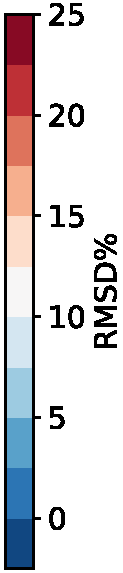
\includegraphics[width=0.0525\textwidth]{img/05271015_wholesky_cb.pdf}}%
\multiput(775,650)(0,80){14}{\line(0,1){40}}
\multiput(570,570)(0,80){14}{\line(0,1){40}}
\put(0,900){(b)}%
\end{overpic}%
\vspace{3mm}
\caption[wholesky05271015]{ETR results of four radiance predictions on holdout test sky 05/27/2013 10:15. (a) shows the camera processed JPG sky capture for convenience (the model was trained on TIFF data). (b) shows RMSD error across the entire sky. Radiance for samples (11), (56), (39) and (74) are pinpointed at their location in the sky. Samples (39) and (74) were the two worst predictions, with RMSD errors of 23.63\% and 21\% respectively.}
\label{fig:wholesky_05271015}
\end{center}
\end{figure}

For the same holdout test sky (05/27/2013 10:15), \autoref{fig:wholesky_05271015} shows ETR prediction error across the entire hemispherical sky, and highlights the two worst spectral radiance predictions (23.63\% and 21\% RMSD). These two measurements occur near the sun's corona, where radiance values are traditionally higher and more erratic than the rest of a clear sky. Two other predictions selected at random are shown for comparison. A vast majority of the 81 samples are predicted to within 1\% RMSD. Note that even with ``high'' error, predicted curves align with ground truth measurements in terms of shape. The models therefore have learned the wavelength relative intensities of the sky in accordance with capture time, sun location, etc. This is consistent with nearly all predicted results; while the magnitudes per wavelength sometimes deviate, the general shapes each predicted curve is accurate.

Although we were expecting some insight from providing multiple exposures of sky images, results seem to indicate that HDR data, at least for clear skies, does not improve model prediction. All HDR runs resulted in very similar error to non-HDR runs. Similarly, differences in results between 0.25 s, 1 s, and 2 s exposures were also insignificant. We believe this may be because clear sky color changes are so ``uniform'' throughout the day, that multiple exposures lack significance. In other words, all provided exposures may have had the same color change trends. We suspect that HDR data will be more significant in the reconstruction of spectral radiance for scattered and overcast skies, as the color variations of clouds are less uniform across exposures.

\begin{figure}[pos=tbp]
\begin{center}
\begin{overpic}[width=0.48\textwidth]{img/results_color_07261315.pdf}
\put(150,610){(a)}%
\end{overpic}%
~%
\begin{overpic}[width=0.48\textwidth]{img/results_color_09241539.pdf}
\put(150,610){(b)}%
\end{overpic}%
\vspace{-1mm}
\caption[resultscolor]{Sky color model made little to no difference in training and prediction results. (a) and (b) show RMSD results on 07/26/2013 13:15 and 09/24/2013 13:15 respectively.}
\label{fig:results_color}
\end{center}
\end{figure}

Results of our color experiment (\autoref{fig:results_color}) seem to indicate that color model is irrelevant to our method. This implies that our method can be used with any representation of color, as the trends in color across the sky are similar regardless of format. It is unclear if using color data initially captured in an sRGB format somehow restricted the range of the other color models after conversion. In other words, would initially capturing the sky in a color model that maps to a larger color space be better?

\begin{figure}[pos=tbp]
\begin{center}
\includegraphics[width=0.55\textwidth]{img/results_resolution.pdf}
\vspace{-2mm}
\caption[resultsresolution]{Limiting resolution to 5 nm drastically decreases model size, improves computation speed, and even increases prediction success, likely because the prediction problem becomes simpler with $^1$/$_5$ the number of radiance values to predict. Further reductions yield diminishing returns.}
\label{fig:results_resolution}
\end{center}
\end{figure}

The results of the spectral resolution experiment (\autoref{fig:results_resolution}) show the benefits of decreasing spectral resolution from 1 to 5 nm. Model sizes (particularly the large ensemble models), as well as model training and prediction times, decrease significantly. The improvements in prediction accuracy are likely due to the radiance curve being more smooth, i.e. fewer peaks and valleys for the regression model to learn, as well as a simpler prediction problem in general, i.e. fewer outputs to predict. The size of the training dataset also decreases with reduced resolution, but that is eclipsed by the largest model sizes. Beyond 5 nm resolution, further reductions result in diminishing returns. This is an important find for real-time applications, which may operate on limited embedded hardware.

We note here that results between the minimally processed, uncompressed TIFF sky images and traditional, camera processed, compressed JPG sky images, were roughly the same (\autoref{fig:results_models}). TIFF data resulted in only slightly better results ($\mathtt{\sim}$1\%) on some skies, though that may be within the standard deviation of prediction error and machine learning random fluctuation. In terms of storage space and processing, the TIFF images ($\mathtt{\sim}$35 MB) are roughly 15 times larger than the JPG images compressed with quality level 100 ($\mathtt{\sim}$2.5 MB). Given the similar results, we recommend the use of JPG captures for real-time applications of our method.

\begin{figure}[pos=tbp]
\begin{center}
\begin{overpic}[width=0.6\textwidth]{img/sradmaps.jpg}%
\put(-55,600){(a)}%
\put(-55,370){(b)}%
\put(-55,120){(c)}%
\put(100,755){(1)}%
\put(350,755){(2)}%
\put(590,755){(3)}%
\put(840,755){(4)}%
\end{overpic}%
%\vspace{-2mm}
\caption[resultssradmapall]{Columns (1-4) are the holdout test skies in \autoref{tab:testskies}, in respective order. Rows (a) and (b) show traditional, camera processed JPG and minimally processed TIFF captures, respectively. Row (c) shows the sradmap visualizations generated for skies in row (b); we use our ETR model to predict spectral radiance (350-1780 nm) for every pixel of test sky image, sum the radiance distribution, and visualize with a false-color map.}
\label{fig:results_sradmapall}
\end{center}
\end{figure}

\begin{figure}[pos=tbp]
\begin{center}
\includegraphics[width=0.25\textwidth]{img/07261315_sradmap_gray.png}%
\hspace{2mm}%
\includegraphics[width=0.25\textwidth]{img/07261315_sradmap.png}%
\hspace{2mm}%
\includegraphics[width=0.1\textwidth]{img/sradmap_cbs.jpg}%
%\vspace{-1mm}
\caption[resultssradmap0726]{False-colored sradmap visualizations for holdout test sky 07/26/2013 13:15. Each pixel plotted is a summation of an entire spectral radiance distribution (350-1780 nm). There is no significance to the summation algorithm; it is simply used to visualize the data.}
\label{fig:results_sradmap_0726}
\end{center}
\end{figure}

Spectral radiance files (sradmaps) are the culminating whole sky output of our methods. They are generated by extracting features per pixel of test skies (\autoref{tab:testskies}) and feeding them through any one of our models. Linear scale false-color visualizations of ETR model predicted sradmaps are shown in \autoref{fig:results_sradmapall} and \autoref{fig:results_sradmap_0726}. Test sky images were first scaled down to a resolution of 333x333 pixels, to anticipate real-time processing speeds. sradmap generation, visualization, and logged output took $\mathtt{\sim}$20 s to complete on the same machine specified in \autoref{ssec:resolution}; embedded hardware would likely take longer. Visualization of sradmap and logged output are not necessary for real-time applications.
\begin{figure}[pos=p]
\begin{center}
\begin{overpic}[width=0.48\textwidth]{img/results_lrt_05261515_135_12.pdf}%
\put(690,250){\includegraphics[width=0.125\textwidth]{img/05261515.jpg}}%
\put(905,455){\linethickness{0.4mm}\color{yellow}\circle{40}}%
\end{overpic}%
~%
\begin{overpic}[width=0.48\textwidth]{img/results_lrt_05271015_135_12.pdf}%
\put(690,250){\includegraphics[width=0.125\textwidth]{img/05271015.jpg}}%
\put(905,455){\linethickness{0.4mm}\color{yellow}\circle{40}}%
\end{overpic}%
% ~%
% \begin{overpic}[width=0.325\textwidth]{img/results_lrt_09241539_135_12.pdf}%
% \put(690,250){\includegraphics[width=0.09\textwidth]{img/09241539.jpg}}%
% \put(920,470){\linethickness{0.3mm}\color{blue}\circle{35}}%
% \end{overpic}%
%\vspace{-2mm}
\caption[lrt3312]{Spectral radiance at (33.75\degree~azimuth, 12.12\degree~altitude), circled, for two of the holdout test skies in \autoref{tab:testskies}. Spectroradiometer measurement, ETR model prediction, and libRadtran estimation plotted.}
\label{fig:lrt_3312}
\end{center}
\end{figure}

\begin{figure}[pos=p]
\begin{center}
\begin{overpic}[width=0.35\textwidth]{img/results_lrt_05271015_292_53.pdf}%
% \put(165,650){(a)}%
\end{overpic}%
%~~~%
\begin{overpic}[width=0.28\textwidth]{img/05271015.jpg}%
\put(250,400){\linethickness{0.25mm}\color{black}\line(-1,0){310}}%11
\put(250,400){\color{black}\circle*{25}}%
% \put(140,445){(a)}%
\put(580,575){\linethickness{0.25mm}\color{black}\line(1,0){550}}%11
\put(580,575){\color{black}\circle*{25}}%
% \put(470,620){(b)}%
\end{overpic}%
%~~~%
\begin{overpic}[width=0.35\textwidth]{img/results_lrt_05271015_135_71.pdf}%
% \put(165,650){(b)}%
\end{overpic}%
%\vspace{-3mm}
\caption[lrt0527]{Spectral radiance for two sky samples of holdout test sky 05/27/2013 10:15. Spectroradiometer measurement, ETR model prediction, and libRadtran estimation plotted.}
\label{fig:lrt_0527}
\end{center}
\end{figure}

\begin{figure}[pos=p]
\begin{center}
\begin{overpic}[width=0.35\textwidth]{img/results_lrt_07261315_292_53.pdf}%
% \put(165,650){(a)}%
\end{overpic}%
%~~~%
\begin{overpic}[width=0.28\textwidth]{img/07261315.jpg}%
\put(250,400){\linethickness{0.25mm}\color{black}\line(-1,0){310}}%11
\put(250,400){\color{black}\circle*{25}}%
% \put(140,445){(a)}%
\put(580,575){\linethickness{0.25mm}\color{black}\line(1,0){550}}%11
\put(580,575){\color{black}\circle*{25}}%
% \put(470,620){(b)}%
\end{overpic}%
%~~~%
\begin{overpic}[width=0.35\textwidth]{img/results_lrt_07261315_135_71.pdf}%
% \put(165,650){(b)}%
\end{overpic}%
%\vspace{-3mm}
\caption[lrt0726]{Spectral radiance for two sky samples of holdout test sky 07/26/2013 13:15. Spectroradiometer measurement, ETR model prediction, and libRadtran estimation plotted. libRadtran computed radiance deviates from both ETR predictions and measured ground truth data, likely because of the lack of needed atmospheric configuration data. Note the existence of cirrus clouds near the horizon.}
\label{fig:lrt_0726}
\end{center}
\end{figure}

\section{Validation}
\label{sec:validation}

First, no samples from our holdout test skies (\autoref{tab:testskies}), chosen at random, were used during training or preliminary testing of any model. Machine learning projects often use this method to validate a model's ability to generalize over unforeseen data. The results presented in \autoref{fig:results_models}, \autoref{fig:results_05271015}, and \autoref{fig:wholesky_05271015} show that our models have this ability. The results of our additional experiments show that our method is robust against implementation details such as image compression, exposure, and color model.

Next, the sradmaps presented in \autoref{fig:results_sradmapall} and \autoref{fig:results_sradmap_0726} are the result of using every pixel per test sky. These maps demonstrate that our models have the ability to generalize across the entire hemisphere (i.e. predict spectral radiance for every point in the sky) even when trained on a mere skeleton of samples (81 concentric 1\degree~steridians). Note that most of the sky is unaccounted for by the skeleton, including points beyond the variance of sun and sky coordinates. sradmaps contain predictions for the entire sky.

Finally, we compare our ETR model predictions along side our ground truth measurements, with the radiance distributions computed by libRadtran \citep{emde_libradtran}, a popular, validated radiative transfer equation (RTE) software package that uses a variety of solvers developed in collaboration over decades and published in peer-reviewed outlets such as: the Journal of Quantitative Spectroscopy \& Radiative Transfer, Atmospheric Measuring Techniques, Atmospheric Chemistry and Physics, Applied Optics, etc. MYSTIC \citep{buras_2011, mayer_2009, mayer_2005} and DISTORT \citep{buras_2011, dahlback_1991, stamnes_1988} are the two primary comprehensive equation solvers which have been validated in multiple international model comparison studies \citep{emde_2015, kokhanovsky_2010, cahalan_2005}. Since 2005, libRadtran has been cited by hundreds of peer-reviewed publications.

libRadtran was configured the same for all four holdout test skies. In other words, no sky-specific data (atmospheric measurements, aerosol databases, parameters, or ranges) were specified per test sky - we used the default configuration. \autoref{fig:lrt_3312} and \autoref{fig:lrt_0527} show that libRadtran spectral radiance for three of our four holdout test skies were in alignment with both ETR model predictions and ground truth measurements. However, for test sky 07/26/2013 13:15, libRadtran deviates from both ETR predictions and ground truth measurements (\autoref{fig:lrt_0726}). All tested samples for this sky show similar deviations in magnitude, but not curve shape. As mentioned, libRadtran requires accurate atmospheric data for its calculations. Because such data was not configured, and because our predictions are closer to ground truth measurements, it is possible that our ETR model learned the sky specific atmospheric conditions libRadtran needed in order to compute accurately. In particular, we note the cirrus clouds along the horizon, which might indicate ice crystals in the atmosphere, and account for deviations between data-driven predictions and physically-based model calculations.

%\clearpage
%\vspace{5mm}

\section{Conclusions}
\label{sec:conclusion}

Whole sky spectral radiance distributions are needed for accurate computations in a variety of applications, and yet they are often oversimplified. Real-time capable models are needed to estimate them to within acceptable tolerances. We presented a solution that: (1) took photographs of the entire hemispherical sky and measured the incoming radiance at various points, (2) used those measurements and modern machine learning methods to train regression models, and (3) used those models to predict atmospheric spectral radiance (350-1780 nm) at 1 nm resolution for the entire sky, given a photo of a clear sky and its capture timestamp, in $\mathtt{\sim}$20 s of processing time, making the solution viable for real-time applications. Our whole sky prediction error, for all four holdout test skies, none of which were used for training, was below 7.5\% RMSD, and most of the predicted spectral radiance distributions were in line with libRadtran.

Our results show that image compression, color model, and exposure of clear sky imagery have little to no effect on our method. This implies that our solution is robust and less likely to be affected by  implementation details. We also showed that our models have the ability to generalize across the hemispherical space between measured sky samples, allowing for atmospheric spectral radiance predictions for every point in a sky image.

Our trained models can be used as-is, with similarly exposed and oriented sky photos. And our methods can be reproduced to train models using new datasets. Various sky scanning systems exist which can be employed to provide regional training data. Existing correlated sky imagery and spectral radiance datasets from around the world can (and should) be used with our method. Once normalized, such comprehensive datasets could lead to even more robust models (e.g. more variations of sky turbidity). As mentioned, aerosol data can also be included as training and prediction features, supplied from local building sensors, GOES satellite measurements, and/or triangulated atmospheric measuring station data. Site location coordinates and/or elevation could also be investigated as input features when using multi-site data. More spectral radiance measurements within the circumsolar region would also likely improve accuracy (clear or cloudy sky), as the bulk of the energy is accounted for within that region of the sky. All research in this area could benefit by a scanning pattern that accounts for this.

Although many downstream applications of our research are possible, one immediately viable option is a building monitoring system equipped with all-sky camera that adjusts smart glazing and kinetic facades in response to spectral radiance across the entire non-occluded sky. Such a system would automatically harness (or attenuate) light and heat with more fine-grain control and accuracy than one that operates on a single downwelling measurement, and would be much more affordable and efficient than a live, continuously operating sky scanning system. As mentioned, various procedural processes can be applied to distinguish clear, scattered, and overcast skies, so that pixels and image regions can be passed to appropriate models for spectral radiance prediction. Cloud detection research regularly separates clear from cloudy portions of skies. We hope our research motivates the building performance community to further refine such a system. We also hope that the graphics (rendering) community notices the useful of our sradmap tool. The predicted spectral radiance distributions can and should be used in spectral renderers (the future of rendering) to provide the most accurate natural day-lighting scenes.

Further work will focus on scattered cloudy skies. Scattered skies account for the bulk of our publicly available dataset (63\%), and in general is more complicated to model. More modern, complex machine-learning techniques, such as neural networks, are likely necessary to model the complex non-linear relationships of scattered skies. Simply throwing our entire dataset (clear, scattered, and overcast data) at a neural architecture search (NAS) deep learning neural network infrastructure, we achieved an 83\% R\textsuperscript{2} score, suggesting there is potential for a unified machine learned model. More investigation is needed to find the right network configuration to handle this problem. We also believe that HDR data will have more of an impact on cloudy versus clear skies, because the color gradients are not nearly as uniform. Additional work should include improving our Gaussian weighted color sampling with rectangular (as opposed to square) convolution kernels, to capture the projected solid angle area (ellipse) precisely.

Portions of this work were presented at SPIE Optics and Photonics for Information Processing XII \citep{delrocco_spie}.

\section*{Acknowledgements}

We would like to acknowledge Dr. Donald P. Greenberg and the Program of Computer Graphics (PCG) at Cornell University for support and open source release of captured sky data; Dr. Steve Marschner for the DSLR; Dr. Harold van Es and Dr. William D. Philpot for ASD spectroradiometer access and discussions; Kevin Pratt, Hurf Sheldon, Lars Schumann, and Daniel Knowlton for various contributions to spectral sky projects; Maik Riechert for raw image processing code and discussions; and Jeremiah Eisenmenger for discussions on hemispherical projections.

% list author credit taxonomy contribution roles tagged using \verb+\credit+ 
% \printcredits

% bibliography
\bibliography{refs}
%\vskip3pt

% Appendix sections are coded under \verb+\appendix+.
%\appendix
%\mbox{}
%\clearpage

% \section*{Appendix A - 05/26/13 15:15 \footnote{Provided for reviewing purposes only.}}

%\begin{strip}
\noindent
Whole sky ETR predictions for holdout test sky {05/26/2013 15:15}.\\%
%\vspace{-10mm}
%\end{strip}

%\begin{strip}
\begin{center}
\includegraphics[width=0.30\textwidth]{img/05261515.jpg}
\includegraphics[width=0.30\textwidth]{img/05261515_sradmap.png}
\includegraphics[width=0.38\textwidth]{img/05261515_wholesky_full.pdf}\\
\vspace{0.26in}%
\includegraphics[width=0.48\textwidth]{img/05261515_measured.pdf}
\includegraphics[width=0.48\textwidth]{img/05261515_predicted.pdf}\\
\vspace{0.2in}%
\includegraphics[width=0.48\textwidth]{img/05261515_std.pdf}
\includegraphics[width=0.48\textwidth]{img/05261515_ratio.pdf}
\end{center}
%\end{strip}

\clearpage
%\begin{strip}
\noindent
15 of 81 consecutive ETR spectral radiance predictions for holdout test sky {05/26/2013 15:15}.\\%
%\vspace{-10mm}
%\end{strip}

%\begin{strip}
\begin{center}
\includegraphics[width=0.325\textwidth]{img/05261515_s29.pdf}
\includegraphics[width=0.325\textwidth]{img/05261515_s30.pdf}
\includegraphics[width=0.325\textwidth]{img/05261515_s31.pdf}\\
\includegraphics[width=0.325\textwidth]{img/05261515_s32.pdf}
\includegraphics[width=0.325\textwidth]{img/05261515_s33.pdf}
\includegraphics[width=0.325\textwidth]{img/05261515_s34.pdf}\\
\includegraphics[width=0.325\textwidth]{img/05261515_s35.pdf}
\includegraphics[width=0.325\textwidth]{img/05261515_s36.pdf}
\includegraphics[width=0.325\textwidth]{img/05261515_s37.pdf}\\
\includegraphics[width=0.325\textwidth]{img/05261515_s38.pdf}
\includegraphics[width=0.325\textwidth]{img/05261515_s39.pdf}
\includegraphics[width=0.325\textwidth]{img/05261515_s40.pdf}\\
\includegraphics[width=0.325\textwidth]{img/05261515_s41.pdf}
\includegraphics[width=0.325\textwidth]{img/05261515_s42.pdf}
\includegraphics[width=0.325\textwidth]{img/05261515_s43.pdf}
\end{center}
%\end{strip}

\mbox{}
\clearpage

% \section*{Appendix B - 05/27/13 10:15 \footnote{Provided for reviewing purposes only.}}

%\begin{strip}
\noindent
Whole sky ETR predictions for holdout test sky {05/27/2013 10:15}.%
%\vspace{-10mm}
%\end{strip}

%\begin{strip}
\begin{center}
\includegraphics[width=0.30\textwidth]{img/05271015.jpg}
\includegraphics[width=0.30\textwidth]{img/05271015_sradmap.png}
\includegraphics[width=0.38\textwidth]{img/05271015_wholesky_full.pdf}\\
\vspace{0.26in}%
\includegraphics[width=0.48\textwidth]{img/05271015_measured.pdf}
\includegraphics[width=0.48\textwidth]{img/05271015_predicted.pdf}\\
\vspace{0.2in}%
\includegraphics[width=0.48\textwidth]{img/05271015_std.pdf}
\includegraphics[width=0.48\textwidth]{img/05271015_ratio.pdf}
\end{center}
%\end{strip}

\clearpage
%\begin{strip}
\noindent
15 of 81 consecutive ETR spectral radiance predictions for holdout test sky {05/27/2013 10:15}.\\%
%\vspace{-10mm}
%\end{strip}

%\begin{strip}
\begin{center}
\includegraphics[width=0.325\textwidth]{img/05271015_s64.pdf}
\includegraphics[width=0.325\textwidth]{img/05271015_s65.pdf}
\includegraphics[width=0.325\textwidth]{img/05271015_s66.pdf}\\
\includegraphics[width=0.325\textwidth]{img/05271015_s67.pdf}
\includegraphics[width=0.325\textwidth]{img/05271015_s69.pdf}
\includegraphics[width=0.325\textwidth]{img/05271015_s70.pdf}\\
\includegraphics[width=0.325\textwidth]{img/05271015_s71.pdf}
\includegraphics[width=0.325\textwidth]{img/05271015_s72.pdf}
\includegraphics[width=0.325\textwidth]{img/05271015_s73.pdf}\\
\includegraphics[width=0.325\textwidth]{img/05271015_s74.pdf}
\includegraphics[width=0.325\textwidth]{img/05271015_s75.pdf}
\includegraphics[width=0.325\textwidth]{img/05271015_s76.pdf}\\
\includegraphics[width=0.325\textwidth]{img/05271015_s77.pdf}
\includegraphics[width=0.325\textwidth]{img/05271015_s78.pdf}
\includegraphics[width=0.325\textwidth]{img/05271015_s79.pdf}
\end{center}
%\end{strip}

\mbox{}
\clearpage

% \section*{Appendix C - 07/26/13 13:15 \footnote{Provided for reviewing purposes only.}}

%\begin{strip}
\noindent
Whole sky ETR predictions for holdout test sky {07/26/2013 13:15}.\\%
%\vspace{-10mm}
%\end{strip}

%\begin{strip}
\begin{center}
\includegraphics[width=0.30\textwidth]{img/07261315.jpg}
\includegraphics[width=0.30\textwidth]{img/07261315_sradmap.png}
\includegraphics[width=0.38\textwidth]{img/07261315_wholesky_full.pdf}\\
\vspace{0.26in}%
\includegraphics[width=0.48\textwidth]{img/07261315_measured.pdf}
\includegraphics[width=0.48\textwidth]{img/07261315_predicted.pdf}\\
\vspace{0.2in}%
\includegraphics[width=0.48\textwidth]{img/07261315_std.pdf}
\includegraphics[width=0.48\textwidth]{img/07261315_ratio.pdf}
\end{center}
%\end{strip}

\clearpage
%\begin{strip}
\noindent
15 of 81 consecutive ETR spectral radiance predictions for holdout test sky {07/26/2013 13:15}.\\%
%\vspace{-10mm}
%\end{strip}

%\begin{strip}
\begin{center}
\includegraphics[width=0.325\textwidth]{img/07261315_s00.pdf}
\includegraphics[width=0.325\textwidth]{img/07261315_s01.pdf}
\includegraphics[width=0.325\textwidth]{img/07261315_s02.pdf}\\
\includegraphics[width=0.325\textwidth]{img/07261315_s04.pdf}
\includegraphics[width=0.325\textwidth]{img/07261315_s05.pdf}
\includegraphics[width=0.325\textwidth]{img/07261315_s06.pdf}\\
\includegraphics[width=0.325\textwidth]{img/07261315_s07.pdf}
\includegraphics[width=0.325\textwidth]{img/07261315_s08.pdf}
\includegraphics[width=0.325\textwidth]{img/07261315_s09.pdf}\\
\includegraphics[width=0.325\textwidth]{img/07261315_s10.pdf}
\includegraphics[width=0.325\textwidth]{img/07261315_s11.pdf}
\includegraphics[width=0.325\textwidth]{img/07261315_s12.pdf}\\
\includegraphics[width=0.325\textwidth]{img/07261315_s13.pdf}
\includegraphics[width=0.325\textwidth]{img/07261315_s14.pdf}
\includegraphics[width=0.325\textwidth]{img/07261315_s15.pdf}
\end{center}
%\end{strip}

\mbox{}
\clearpage

% \section*{Appendix D - 09/24/13 15:39 \footnote{Provided for reviewing purposes only.}}

%\begin{strip}
\noindent
Whole sky ETR predictions for holdout test sky {09/24/2013 15:39}.\\%
%\vspace{-10mm}
%\end{strip}

%\begin{strip}
\begin{center}
\includegraphics[width=0.30\textwidth]{img/09241539.jpg}
\includegraphics[width=0.30\textwidth]{img/09241539_sradmap.png}
\includegraphics[width=0.38\textwidth]{img/09241539_wholesky_full.pdf}\\
\vspace{0.26in}%
\includegraphics[width=0.48\textwidth]{img/09241539_measured.pdf}
\includegraphics[width=0.48\textwidth]{img/09241539_predicted.pdf}\\
\vspace{0.2in}%
\includegraphics[width=0.48\textwidth]{img/09241539_std.pdf}
\includegraphics[width=0.48\textwidth]{img/09241539_ratio.pdf}
\end{center}
%\end{strip}

\clearpage
%\begin{strip}
\noindent
15 of 81 consecutive ETR spectral radiance predictions for holdout test sky {09/24/2013 15:39}.\\%
%\vspace{-10mm}
%\end{strip}

%\begin{strip}
\begin{center}
\includegraphics[width=0.325\textwidth]{img/09241539_s00.pdf}
\includegraphics[width=0.325\textwidth]{img/09241539_s01.pdf}
\includegraphics[width=0.325\textwidth]{img/09241539_s02.pdf}\\
\includegraphics[width=0.325\textwidth]{img/09241539_s03.pdf}
\includegraphics[width=0.325\textwidth]{img/09241539_s04.pdf}
\includegraphics[width=0.325\textwidth]{img/09241539_s05.pdf}\\
\includegraphics[width=0.325\textwidth]{img/09241539_s06.pdf}
\includegraphics[width=0.325\textwidth]{img/09241539_s07.pdf}
\includegraphics[width=0.325\textwidth]{img/09241539_s08.pdf}\\
\includegraphics[width=0.325\textwidth]{img/09241539_s09.pdf}
\includegraphics[width=0.325\textwidth]{img/09241539_s10.pdf}
\includegraphics[width=0.325\textwidth]{img/09241539_s11.pdf}\\
\includegraphics[width=0.325\textwidth]{img/09241539_s12.pdf}
\includegraphics[width=0.325\textwidth]{img/09241539_s13.pdf}
\includegraphics[width=0.325\textwidth]{img/09241539_s14.pdf}
\end{center}
%\end{strip}

\mbox{}
\clearpage


% \bio{}
% Author biography without author photo.
% \endbio

\end{document}
